\documentclass[sigconf]{acmart}

\settopmatter{
printacmref=false,
printccs=false,
printfolios=false
}

\renewcommand\footnotetextcopyrightpermission[1]{}

\pagestyle{plain}

\pagenumbering{arabic}

\fancyhf{}

\renewcommand\shortauthors{}

\acmConference{}{}{}
\acmBooktitle{}
\acmPrice{}
\acmDOI{}
\acmISBN{}

\usepackage{graphicx}


\begin{document}

\title{Collecting and Analyzing Multidimensional Data under Local Differential Privacy}

\author{Nabeel Navab}
\affiliation{
\institution{Institute of IT Security, University of Lübeck}
\city{Lübeck}
\country{Germany}
}
\email{nabeel.navab@student.uni-luebeck.de}

\begin{abstract}
The increasing collection of user data by online services and smart devices has raised significant concerns regarding privacy preservation. Local Differential Privacy (LDP), a privacy model that perturbs data on a user's device before transmission, has emerged as a promising approach for protecting sensitive information while still enabling data analysis. However, applying LDP to multidimensional datasets remains challenging because the utility of collected data often decreases as the number of attributes grows.This paper examines a multidimensional LDP framework that introduces the Piecewise Mechanism (PM) and Hybrid Mechanism (HM) to improve the accuracy of statistical estimation under strong privacy guarantees. Furthermore, the framework extends LDP techniques to machine learning tasks through privacy-preserving stochastic gradient descent. Experimental results demonstrate that the proposed methods achieve higher utility than existing approaches while maintaining rigorous privacy protection, making them suitable for large-scale data collection and analysis.



\end{abstract} 
\keywords{
Local Differential Privacy,
Multidimensional Data,
Privacy Preservation,
Statistical Analysis,
Machine Learning
}

\maketitle

\section{Introduction}

Differential Privacy (DP) protects individual records by limiting the information that can be inferred from published data~\cite{dwork2006}, while Local Differential Privacy (LDP) applies this protection directly on the user's device before data collection. LDP enables the collection of user data while preserving privacy by perturbing information before it is transmitted to a data collector.
 Although existing LDP mechanisms provide strong privacy guarantees, they are primarily designed for single-dimensional data and often suffer from significant utility degradation when applied to multidimensional datasets.Practical deployments of LDP have also been explored in systems such as RAPPOR~\cite{rappor2014}, which applies randomized response techniques for privacy-preserving data collection.


In practical applications, user records frequently contain multiple numerical and categorical attributes.The framework supports both numerical and categorical attributes, which require different perturbation and estimation strategies under LDP.
 Collecting and analyzing such data under LDP presents a fundamental challenge, as the privacy budget must be distributed across several dimensions, increasing noise and reducing estimation accuracy. Consequently, designing mechanisms that preserve both privacy and utility for multidimensional data has become an important research problem.

In \textit{Collecting and Analyzing Multidimensional Data with Local Differential Privacy}, Wang et al. address this challenge by proposing a framework for multidimensional data collection and analysis under LDP. The framework introduces the Piecewise Mechanism (PM) and Hybrid Mechanism (HM), which improve statistical estimation while maintaining formal privacy guarantees. Furthermore, the framework extends LDP techniques to machine learning through privacy-preserving stochastic gradient descent. Experimental results demonstrate improved utility compared to existing LDP methods across a variety of statistical and machine learning tasks.



\section{The Multidimensional LDP Framework}
The multidimensional LDP framework presented in~\cite{wang2019} addresses a key limitation of traditional LDP mechanisms, which often experience substantial utility loss when applied to datasets containing multiple attributes.

 As the dimensionality of the data increases, perturbing every attribute independently introduces excessive noise and reduces the accuracy of statistical analysis.

The framework follows a client-side privacy model in which each user perturbs their data locally before transmission. For multidimensional records, the privacy budget is carefully allocated across attributes to limit utility loss while maintaining the desired privacy guarantees. The perturbed reports are then collected by an aggregator, which reconstructs statistical properties of the original dataset through unbiased estimation techniques. This design enables accurate analysis without requiring access to raw user data.

Local Differential Privacy is formally defined by

\begin{equation}
P[M(x)=y] \leq e^{\epsilon} P[M(x')=y]
\end{equation}

for any two possible inputs $x$ and $x'$ and any output $y$, where $\epsilon$ denotes the privacy budget. Smaller values of $\epsilon$ provide stronger privacy guarantees but typically reduce the utility of the collected data.

A central challenge of multidimensional LDP is the allocation of the privacy budget across multiple attributes. When the available privacy budget is divided among several dimensions, each attribute receives a smaller share of the budget, increasing perturbation noise and reducing estimation accuracy. Consequently, utility decreases as the dimensionality of the dataset grows, motivating the need for specialized multidimensional mechanisms.
The impact of dimensionality on estimation accuracy can be expressed through the variance relationship
\begin{equation}
Var[\hat{\mu}] \propto \frac{d}{n\epsilon^2}
\end{equation}
This relationship illustrates that estimation variance increases with the dimensionality $d$ of the dataset and decreases with the number of users $n$ and the privacy budget $\epsilon$. Consequently, multidimensional datasets become increasingly difficult to analyze accurately under strict privacy constraints, motivating the need for mechanisms such as PM and HM.
The central objective of the framework is to reduce the utility degradation introduced by multidimensional perturbation while preserving rigorous local privacy guarantees.

To address the utility degradation associated with multidimensional perturbation, the framework introduces two perturbation mechanisms: the Piecewise Mechanism (PM) and the Hybrid Mechanism (HM)
. PM perturbs numerical values within a carefully designed output range, reducing estimation variance while satisfying the privacy guarantees of LDP. Building on this idea, HM combines multiple perturbation strategies to achieve a more favorable privacy-utility trade-off across different privacy budgets.

The Hybrid Mechanism was designed to combine the advantages of different perturbation strategies, allowing it to maintain high utility across a broader range of privacy budgets than individual mechanisms alone. Experimental results indicate that HM consistently achieves competitive performance across varying privacy settings, making it effective across a wide range of privacy requirements.


The mechanisms primarily target accurate statistical estimation, enabling aggregate properties such as means and distributions to be reconstructed from privatized reports without revealing individual user records.



Figure~\ref{fig:framework} illustrates the core components of the multidimensional LDP framework and the relationship between its perturbation mechanisms and downstream analytical tasks.

\begin{figure}[ht]
\centering
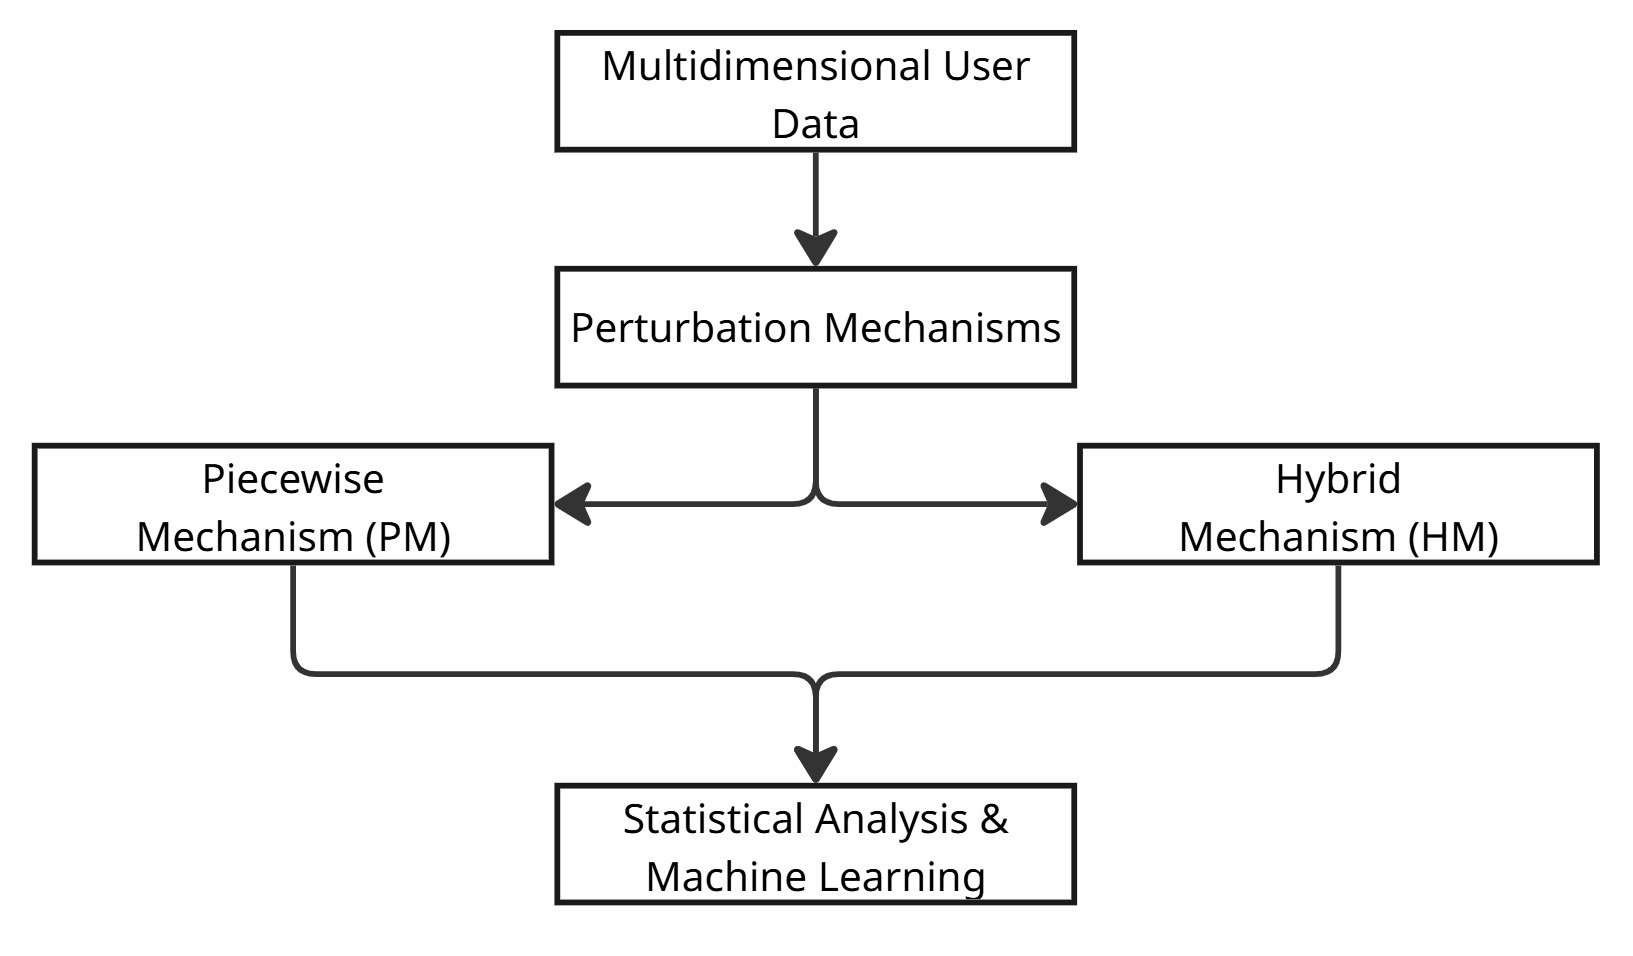
\includegraphics[width=0.9\columnwidth]{framework_workflow.jpg}
\caption{Overview of the multidimensional LDP framework proposed by Wang et al. The framework applies privacy-preserving perturbation through the Piecewise Mechanism (PM) and Hybrid Mechanism (HM) to enable statistical analysis and machine learning on multidimensional data.}
\label{fig:framework}
\end{figure}

In addition to statistical estimation, the framework supports machine learning applications through privacy-preserving stochastic gradient descent (LDP-SGD). Instead of transmitting raw gradients, users locally perturb their updates before sharing them with the server. This enables model training on sensitive multidimensional data without exposing individual records.The integration of perturbation mechanisms with privacy-preserving stochastic gradient descent enables machine learning on sensitive multidimensional datasets while maintaining formal privacy guarantees.




\section{Experimental Evaluation}

 Experimental evaluation on real-world datasets compared the proposed mechanisms against existing LDP approaches under varying privacy budgets and dimensionalities.In addition, the evaluation examined the performance of privacy-preserving machine learning using stochastic gradient descent on perturbed data.


The evaluation considered both numerical and multidimensional datasets to investigate how the mechanisms behave as dimensionality increases. The evaluation measured estimation error under varying privacy budgets and compared PM and HM against existing state-of-the-art LDP approaches.
 This experimental setup allowed the effectiveness of the proposed mechanisms to be assessed under realistic privacy and utility constraints.

In addition to estimation accuracy, the experiments examined the applicability of the framework to privacy-preserving machine learning. The results indicate that the LDP-SGD approach can train useful models while maintaining the privacy guarantees required by local differential privacy, demonstrating the practicality of the framework beyond traditional statistical analysis tasks.

The results demonstrate that both the Piecewise Mechanism
(PM) and Hybrid Mechanism (HM) achieve significantly lower estimation
error than traditional LDP mechanisms. In particular, HM
consistently provides a favorable balance between privacy protection and
utility across a wide range of privacy settings. The
experiments further show that the proposed LDP-SGD framework
enables effective model training while maintaining formal privacy
guarantees.

Overall, the evaluation confirms that the multidimensional LDP framework improves utility while preserving strong privacy guarantees. The results further indicate that carefully designed perturbation and estimation mechanisms can substantially reduce the utility degradation commonly associated with high-dimensional LDP settings.




% \section{Discussion}
%
% Analyze the feasibility of the proposed approach.
%
% Discuss:
%
% \begin{itemize}
% \item Scalability
% \item Security implications
% \item Limitations
% \item Future research directions
% \end{itemize}

\section{Conclusion}

This paper examined a multidimensional Local Differential Privacy framework for privacy-preserving data collection and analysis.
 The framework addresses the challenge of collecting and analyzing multidimensional user data while preserving strong privacy guarantees. Through the Piecewise Mechanism (PM), Hybrid Mechanism (HM), and privacy-preserving stochastic gradient descent, the proposed approach improves the utility of statistical estimation and machine learning compared to conventional LDP methods. Experimental results demonstrate that the framework achieves a favorable balance between privacy protection and data utility across multidimensional datasets. The work represents an important step toward practical privacy-preserving data collection and highlights the potential of LDP for large-scale statistical analysis and machine learning applications.


\bibliographystyle{ACM-Reference-Format}
\bibliography{references}

\end{document}
